% Ergebnisse und Analyse.tex

% Ergebnisse und Analyse Diagramme.tex

\newcommand{\MergesortMesswerte}{%
    \addplot[blue, mark=*] coordinates {
            (25000000,3017372600)
            (50000000,6315632400)
            (100000000,12777405700)
            (200000000,27203738300)
            (400000000,56441153000)
        };
    \addlegendentry{Mergesort}
}

\newcommand{\QuicksortMesswerte}{%
    \addplot[green, mark=*] coordinates {
            (25000000,1528071600)
            (50000000,3248990900)
            (100000000,6653966800)
            (200000000,13778762100)
            (400000000,29074726600)
        };
    \addlegendentry{Quicksort}
}

\newcommand{\GrundlegendeLaufzeitenAbhaengigVonDerArraygroesseDiagrammA}{%
    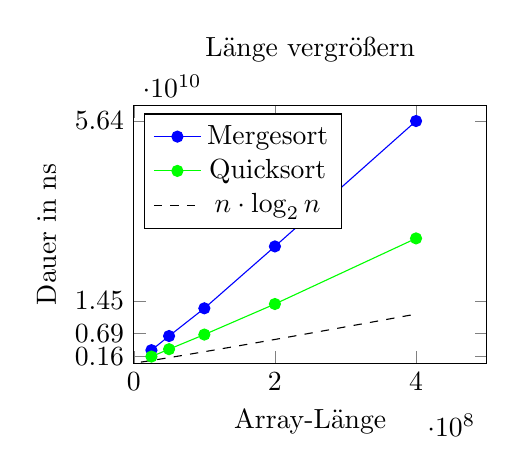
\begin{tikzpicture}
        \begin{axis}[
                title style={yshift=1.5ex},
                width=0.5\textwidth,
                height=0.4\textwidth,
                xlabel={Array-Länge},
                ylabel={Dauer in ns},
                title={Länge vergrößern},
                xmin=0, xmax=5 * 10^8,
                ymin=0*10^6, ymax=6*10^10,
                grid style=dashed,
                legend pos=north west,
                ytick={1609541400,6854920900,14495472700,56441153000},
                % xtick={2^21,2^23,2^24,2^25},
                % xticklabels={$2^{21}$, $2^{23}$, $2^{24}$, $2^{25}$},
                % scaled x ticks=false,
                % scaled y ticks=false,
            ]
            \MergesortMesswerte
            \QuicksortMesswerte
            % n*log2(n)
            \addplot[black, dashed,domain=1e7:4e8, samples=100] {x*log2(x)};
            \addlegendentry{$n \cdot \log_2 n$}
            % % n
            % \addplot[red, dashed,domain=1e7:4e8, samples=100] {x};
            % \addlegendentry{$n$}
            % % log2(n)
            % \addplot[green, domain=1e7:4e8, samples=100] {log2(x)};
            % \addlegendentry{$\log_2 n$}
        \end{axis}
    \end{tikzpicture}%
}

\newcommand{\GrundlegendeLaufzeitenAbhaengigVonDerArraygroesseDiagrammB}{%
    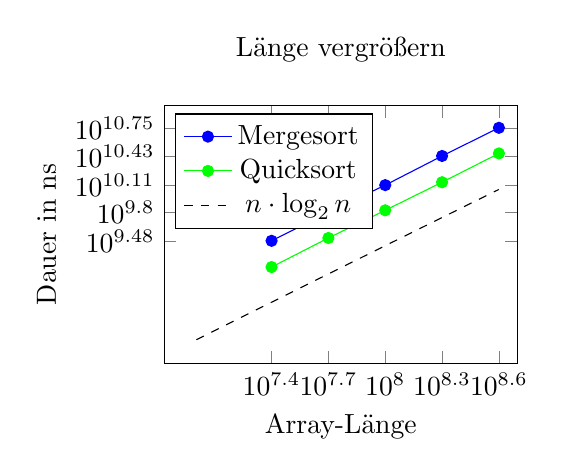
\begin{tikzpicture}
        \begin{axis}[
                title style={yshift=1.5ex},
                width=0.5\textwidth,
                height=0.4\textwidth,
                xlabel={Array-Länge},
                ylabel={Dauer in ns},
                title={Länge vergrößern},
                xmin=0, xmax=5 * 10^8,
                ymin=0*10^6, ymax=1*10^11,
                grid style=dashed,
                legend pos=north west,
                xmode=log,
                log basis x=10,
                xtick=data,
                ymode=log,
                log basis y=10,
                ytick=data,
                % xtick={2^21,2^23,2^24,2^25},
                % xticklabels={$2^{21}$, $2^{23}$, $2^{24}$, $2^{25}$},
                % scaled x ticks=false,
                % scaled y ticks=false,
            ]
            \MergesortMesswerte
            \QuicksortMesswerte
            % n*log2(n)
            \addplot[black, dashed,domain=1e7:4e8, samples=100] {x*log2(x)};
            \addlegendentry{$n \cdot \log_2 n$}
        \end{axis}
    \end{tikzpicture}%
}


% Definiere Variablen
% \newcommand{\Messziel}{Messziel}

% % ----------------------
% % 4. Ergebnisse und Analyse
% % ----------------------
% \newpage
% \chapter{Ergebnisse und Analyse}
% \section{Grundlegende Laufzeiten abhängig von der Arraygröße}
% \subsection{Messziel} % Einleitung
% \subsection{Erwartung}
% \subsection{Diagramm}
% \subsection{Analyse und Interpretation}
% \newpage
% \section{Einfluss des Listentyps} % Listentyps: Zufall, Sortiert, InvertiertSortiert, FastSortiert, Dupliziert
% \subsection{Messziel} % Einleitung
% \subsection{Erwartung}
% \subsection{Diagramm}
% \subsection{Analyse und Interpretation}
% \newpage
% \section{Einfluss der Arraygröße im Detail}
% \subsection{Messziel} % Einleitung
% \subsection{Erwartung}
% \subsection{Diagramm}
% \subsection{Analyse und Interpretation}
% \newpage
% \section{Tiefenbasierte Thread-Erzeugung}
% \subsection{Messziel} % Einleitung
% \subsection{Erwartung}
% \subsection{Diagramm}
% \subsection{Analyse und Interpretation}
% \newpage
% \section{Workerthreads}
% \subsection{Messziel} % Einleitung
% \subsection{Erwartung}
% \subsection{Diagramm}
% \subsection{Analyse und Interpretation}
% \newpage
% \section{Vergleich der Threading-Methoden}
% \subsection{Messziel} % Einleitung
% \subsection{Erwartung}
% \subsection{Diagramm}
% \subsection{Analyse und Interpretation}
% \newpage
% \section{Einfluss des Datentyps der Liste} % Listenart: int, string
% \subsection{Messziel} % Einleitung
% \subsection{Erwartung}
% \subsection{Diagramm}
% \subsection{Analyse und Interpretation}
% % \section{Debug Vs Release}

% % ----------------------
% % 4. Ergebnisse und Analyse
% % ----------------------
% \chapter{Ergebnisse und Analyse}
% \section{Grundlegende Laufzeiten abhängig von der Arraygröße}

% \subsection{Messziel} % Einleitung
\newcommand{\GrundlegendeLaufzeitenAbhaengigVonDerArraygroesseMessziel}{
    Das Messziel besteht darin, die Abhängigkeit des seriellen Algorithmus von der Arraygröße grafisch darzustellen.
    Dadurch können diese Ergebnisse später mit den nicht-seriellen Varianten verglichen werden.
    Gleichzeitig dient dies als einfacher Einstieg in das Thema.
}

% \subsection{Erwartung}
\newcommand{\GrundlegendeLaufzeitenAbhaengigVonDerArraygroesseErwartung}{
    Da die durchschnittliche Laufzeit \(O(n \log n)\) beträgt, erwarte ich eine logarithmische Laufzeiterhöhung bei wachsender Arraygröße.
}
% \subsection{Diagramm}
\newcommand{\GrundlegendeLaufzeitenAbhaengigVonDerArraygroesseDiagramm}{
    \GrundlegendeLaufzeitenAbhaengigVonDerArraygroesseDiagrammA
    \GrundlegendeLaufzeitenAbhaengigVonDerArraygroesseDiagrammB
    \newline
    \GrundlegendeLaufzeitenAbhaengigVonDerArraygroesseDiagrammC
}
% \subsection{Analyse und Interpretation}
\newcommand{\GrundlegendeLaufzeitenAbhaengigVonDerArraygroesseAnalyse}{
    In den ersten 2 Diagram sieht man die Lautzeit verändenderung wenn man Die Listengöße 5 mal verdopelt und bei der 2.5*10^7 startet.
    Bei den 2ersn siht man Die achen logarimsich dargestetl wel es so einfacher ist die Lautzieten anzuzeigen und zu vergleichen.
    Unter disen beiden digramm ist ein 3 wo man die gemese laufzeit Logarisch dargest sihct und für den gößen bereich 1-800000 abgezeigt wird.
    An disen Diagrammen kan man deutlisch ablesen das Mergsot wie qiksortt wirklich eine laufzeit von O(T(n)) = n*log(n) haben.
    Man sihet ebenfalss deutlisch das Mergsot rund dopelt solange braucht wie Qiksoert und das qiksort rund 2*n*log2(n) als laufzeit hatt. Aus disen rundungen kan man ableiten das artizoniren eigentich 2n als lautzietz hatt sowue das der Mergschrit eigentlich 4n als laufzeit hatt. Aber der einfachalb halber bleic ich bei beiden bei n.
    Da man eine linare Laufzeit leichter auf einen blick interpetiren kann habe ich aich die funktion 32n eingezeichet. Und man kan daran ablesen das für ustern zahleberch 1-4*10^8 sogar enie genauere abschäötzung sit als nur n*log2(n).
}